\documentclass[UTF8,12pt,a4paper,fontset=none]{ctexart}
\usepackage{amsmath,amssymb}
\usepackage{booktabs,longtable,array}
\usepackage{geometry}
\usepackage{graphicx}
\usepackage[hidelinks]{hyperref}
\usepackage{url}
\def\UrlBreaks{\do\/\do\_\do\-\do\.\do\a\do\b\do\c\do\d\do\e\do\f\do\g\do\h\do\i\do\j\do\k\do\l\do\m\do\n\do\o\do\p\do\q\do\r\do\s\do\t\do\u\do\v\do\w\do\x\do\y\do\z\do\A\do\B\do\C\do\D\do\E\do\F\do\G\do\H\do\I\do\J\do\K\do\L\do\M\do\N\do\O\do\P\do\Q\do\R\do\S\do\T\do\U\do\V\do\W\do\X\do\Y\do\Z}
\usepackage{fancyhdr}
\usepackage{caption}
\geometry{left=2.5cm,right=2.5cm,top=2.5cm,bottom=2.5cm}
\setmainfont{SimSun}[BoldFont=SimSun,BoldFeatures={FakeBold=3},ItalicFont=SimSun,ItalicFeatures={FakeSlant=0.2}]
\setsansfont{SimSun}[BoldFont=SimSun,BoldFeatures={FakeBold=3}]
\setmonofont{SimSun}[Scale=0.95,BoldFont=SimSun,BoldFeatures={FakeBold=3}]
\setCJKmainfont{SimSun}[BoldFont=SimSun,BoldFeatures={FakeBold=3},ItalicFont=SimSun,ItalicFeatures={FakeSlant=0.2}]
\setCJKsansfont{SimSun}[BoldFont=SimSun,BoldFeatures={FakeBold=3}]
\setCJKmonofont{SimSun}[BoldFont=SimSun,BoldFeatures={FakeBold=3}]
\linespread{1.20}
\setlength{\parindent}{2em}
\setlength{\parskip}{0.15em}
\setlength{\headheight}{15pt}
\setlength{\emergencystretch}{2em}
\raggedbottom
\fancypagestyle{plain}{\fancyhf{}\fancyfoot[C]{\small\thepage}\renewcommand{\headrulewidth}{0pt}}
\pagestyle{fancy}
\fancyhf{}
\fancyfoot[C]{\small\thepage}
\renewcommand{\headrulewidth}{0pt}
\ctexset{section={format=\centering\zihao{3},beforeskip=1.3em,afterskip=.8em},subsection={format=\zihao{4},beforeskip=1em,afterskip=.5em},subsubsection={format=\zihao{-4},beforeskip=.8em,afterskip=.4em}}
\captionsetup{font=small,labelfont=bf}
\hypersetup{pdftitle={基于符号因子联合研究与约束组合优化的 Wingman 系统设计},pdfauthor={Wingman项目资料整理}}
\newcommand{\keywords}[1]{\par\noindent\textbf{关键词：}#1}
\renewenvironment{abstract}{\begin{center}{\zihao{4} 摘\quad 要}\end{center}}{\par}
\begin{document}
\thispagestyle{plain}
\begin{center}
{\zihao{2} 基于符号因子联合研究与约束组合优化的 Wingman 系统设计\par}
\vspace{1em}
\end{center}
\begin{abstract}

针对量化研究中因子构造、预测评价与账户配置相互脱节，以及人工选股偏好难以转化为可执行组合的问题，本文设计并说明 Wingman 日频量化研究与辅助配置系统。系统以点时沪深300成分为研究和评分范围，采用“\textbf{可审计数据-候选因子与符号公式-联合筛选与拟合-全池评分-用户白名单-组合优化-执行复核}”的处理流程，将共享预测能力与用户投资范围分开建模。


在数据层，依据输入可用时点构建历史面板，采用次日开盘执行标签、交易状态账本及开发集与封存测试集隔离，控制未来信息泄漏。在研究层，利用本地栈式虚拟机执行候选表达式，通过内层前向选择、回删和有限配对寻找互补因子，使用固定 LightGBM 模型拟合，并以\textbf{外层时间滚动验证}评价完整选择流程。在配置层，将股票排名分数校准为同周期预期超额收益及估计误差，再结合收缩协方差、交易费用、持仓状态与白名单约束求解目标权重。配置模型设置单股5\%、行业30\%的目标上限；所选股票的成功推荐目标须满足用户指定的正下限，无法满足时明确报告不可行。


截至2026年9月17日，代码注册了65项基础因子，另实现8项沪深300上下文候选特征；离线示例已生成300只合成证券的评分，并贯通名单保存、收益风险估计、配置与观察记录。已有配置回放包含3种方法与3档成本形成的9组工程场景，但每组仅5个交易日、一个折及一个相位，结果为“证据不足”。目前，Wingman已经能在模拟数据上跑通主要流程，但还没有足够的真实市场测试证明策略有效。本文进一步说明当前因子口径、关键参数、异常处理及验证边界，为后续真实样本外研究提供可复现的设计基础。


\keywords{因子研究；符号公式；时间序列验证；LightGBM；组合优化；用户白名单}\end{abstract}\clearpage

\section{问题重述}

\subsection{研究背景与 Wingman 的用途}

量化研究通常包含数据整理、特征构造、预测建模、股票排序与组合配置等步骤。单独完成某一步，并不能回答用户最终关心的“哪些股票可以纳入自己的范围、各分配多少资金、应保留多少现金、当前是否值得调仓”。例如，股票的模型评分较高，只表明其在某一评分口径下相对靠前；评分本身既不是预期收益百分比，也不是账户仓位。


Wingman 的用途是把上述步骤连接为可追溯的研究与辅助配置流程。沪深300在系统中承担基础股票池、全池横截面比较和市场风险参照的作用。系统先计算当期成员的评分，再由用户从展示的股票中自主选择白名单，最后仅在该选择范围内形成新的目标配置。研究目标没有要求复制沪深300权重，也没有设定指数跟踪误差最小化目标。（见支撑材料S1）


本文讨论的是日频研究与离线辅助配置：信号依据收盘后已可获得的信息形成，计划在下一交易日开盘执行。系统不输出精确未来股价，也不把页面生成的方案视为已经成交。当前已有离线工程版本，真实市场联合研究、正式建议开放与连续影子账户仍需分别完成验证。


\subsection{需要解决的问题}

根据设计对话及当前实现，可将任务归纳为四个相互衔接的问题。


第一，如何构建当时确实可得的数据，使历史成员、行业变更、公司行动与交易状态按正确时点进入研究，并将不能成交的事实保留在收益账本中。


第二，如何由现有因子及受控公式提案构成候选，评价因子之间的互补关系，同时控制搜索次数和时间泄漏，使候选筛选与最终评价相互隔离。


第三，如何从模型输出得到\textbf{可解释的股票排序}，再将用户保存的白名单转换为收益、风险、成本共同约束下的\textbf{目标权重、现金与调仓方案}。


第四，如何区分功能运行成功、研究假设通过、正式建议获准与实际执行完成，建立可回放的证据链，而不把演示结果扩写成未经验证的收益结论。


\subsection{输入、输出与研究范围}

数据输入包括历史原始行情、成交量及成交额、历史指数成员与权重、带有效区间的行业分类、公司行动、方向性交易状态，以及独立的收益标签。账户侧输入包括白名单版本、最低目标权重、总预算、持仓和可卖数量；有账户金额时还包括交易单位、费率与容量信息。


研究输出包括公式与因子版本、逐折选择记录、外层评分、验证报告及状态。配置输出包括推荐权重、情景权重范围、现金、收益估计及误差、行业与波动暴露、费用、调仓差额及条件执行结果。所有输出均须绑定数据、模型、配置和名单版本。本文以当前工作区实现为截面，主要依据冻结协议、S2联合研究设计和2026年9月17日的配置实现记录。（见支撑材料S2、S3、S4）


\section{问题分析与设计流程}

\subsection{将预测、决策与执行分开建模}

从数据到交易，中间存在三个不同的数学对象。因子是由历史输入计算得到的特征值；预测评分是模型对股票相对机会的表达；组合权重则是整套账户约束下的决策变量。若把这三者直接等同，就会出现“高分即重仓”“收益率即买入概率”或“目标仓位即实际仓位”等解释错误。


因此，Wingman 采用分层结构。研究层寻找可在\textbf{多只股票上共享的公式与模型}；评分层在统一股票池中比较并得到排行；用户白名单决定允许参与配置的集合；配置层联合考虑收益、风险与费用；执行复核层根据当时条件检查配置方案能否执行。Wingman没有自动下单或成交功能，实际交易由用户自行完成。图\ref{fig:flow}给出各层的输入输出关系。研究评价向候选生成反馈的是允许使用的摘要证据，账户执行事实不反向修改已经冻结的历史信号。


\begin{figure}[htbp]\centering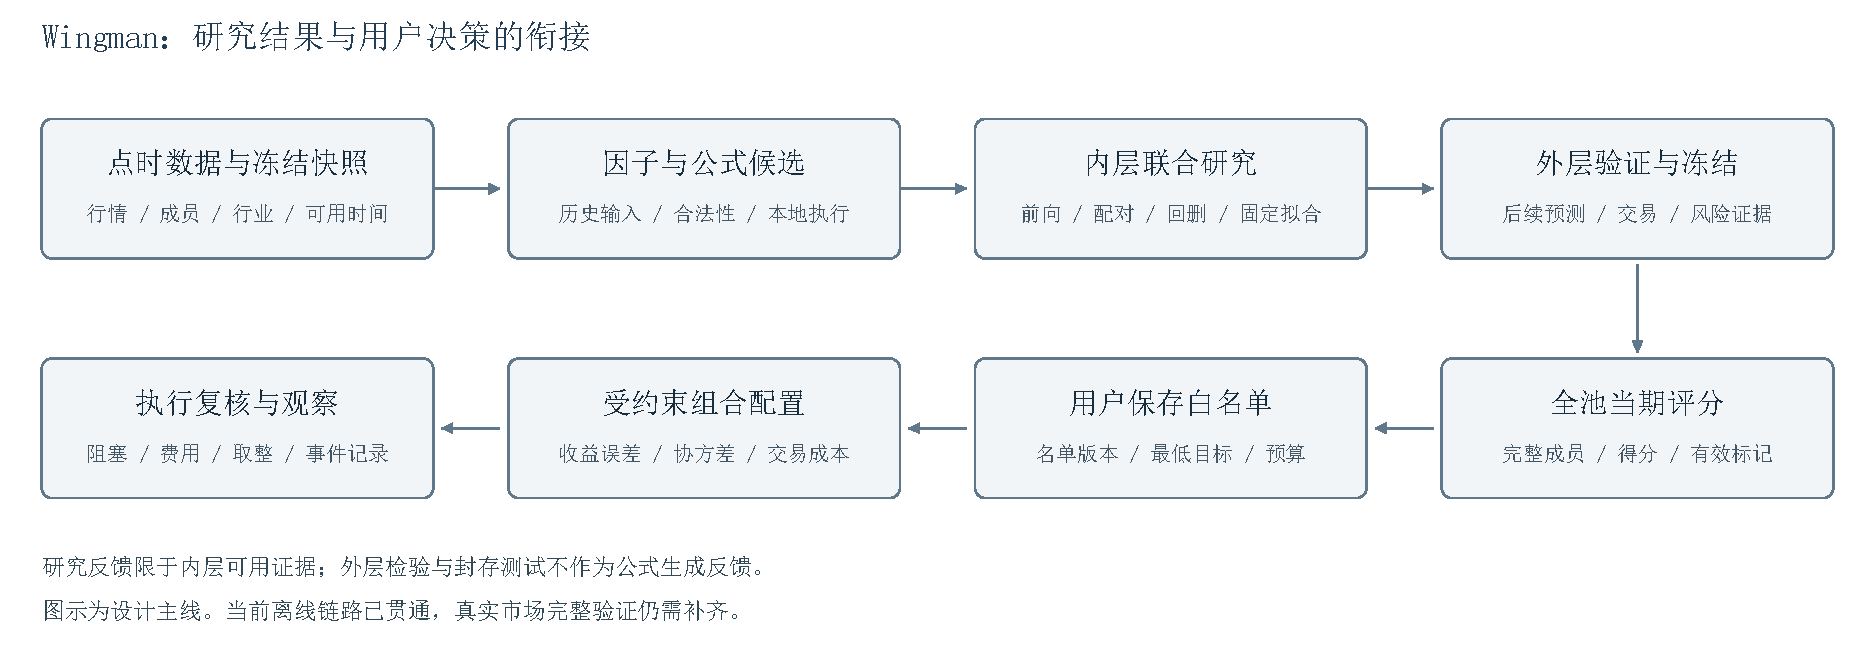
\includegraphics[width=\linewidth]{figs/wingman_flow.pdf}\caption{Wingman的研究与配置流程}\label{fig:flow}\end{figure}
\subsection{市场、行业与个股的职责}

市场层主要控制组合总风险预算与现金空间；行业层主要描述行业环境、行业风险预算及集中度；个股层负责相对机会、横截面排名及收益估计。设计上不把相同的市场分数同时加到每只股票、再次写入决策总分、又在配置时重复放大风险预算。（见支撑材料S1、S2）


\textbf{行业共同上涨也不能直接解释为个股独立能力}。为减少目标股票对自身参照的机械影响，部分市场、行业候选采用剔除自身的同伴基准。当前配置版本使用固定用户预算及行业硬限额，还没有实现经过验证的自动择时或行业预测。


\subsection{研究思路的改变}

原研究路线先用三个简单信号构造参考组合，比较1日、3日和5日周期；达到开发集门槛后，再进入复杂公式研究。其目的在于先检验数据和交易假设，而不是投入大量搜索。已有旧路线结果保留：v1为保留1日基线，v2为证据不足，v3为失败；新设计没有追溯改写这些结论。（见支撑材料S2、S3）


后续设计改为将阶段4、5合并为S2联合研究。其出发点是：\textbf{单因子表现弱，并不意味着与其他因子组合后没有增量}。因此，新流程允许因子在\textbf{内层联合选择}、配对、回删与拟合，再由\textbf{外层检验}整个选择过程。调整的是研究顺序，开发集、外层评价和最终封存测试集的角色仍须分开。


这一变化也改变了评价对象：研究要证明的是“同一套预先规定的选择流程能够产生可靠的后续预测与组合”，而不只是“某一个被挑中的因子在已看过的数据中表现较好”。有限配对只能发现预算范围内的互补关系，不能保证找到全部高阶交互或全局最优因子组。


\subsection{方法选型依据}

RD-Agent-Quant研究将因子与模型的研发组织为提出假设、实现、评价和反馈的迭代过程，为本文组织候选提案与本地评价提供方法参考。\cite{r5}


符号公式适合保留可读的计算结构，但候选是否合法、是否具有预测价值，需要分别验证。\textbf{LightGBM} 可用于刻画特征之间的非线性关系，作为固定的因子组评价与拟合器。\cite{r1}


当证券数量较多、有效历史周期有限时，直接使用样本协方差容易产生不稳定风险估计，因此配置层采用\textbf{收缩协方差}。收益、风险与比例成本可统一写入凸优化目标，使用户选择和资金约束具有明确的可行性含义。\cite{r2,r3} 这些经典方法服务于系统的具体分工，本文不将算法组合本身宣称为已验证的性能创新。


\section{模型假设}

假设一：\textbf{研究时点只能使用当时已可获得的数据}。历史输入的披露、可用和生效时间能够保存或按明确的保守政策推导；缺少可靠时间依据的字段不因日期相同而自动放行。


假设二：正式沪深300研究以历史点时成分为股票池，以冻结快照为输入。样本起点按照当前协议取2014年1月2日；更早原始请求只用于覆盖审计，不自动并入本轮研究。合成演示中的历史日期仅为人工时间轴，与正式市场样本范围无关。


假设三：\textbf{日频信号在第t日完整输入可用后形成，计划于第t+1个交易日开盘执行}。实际成交还需通过方向性交易检查；停牌、涨跌停或报价缺失不被假设为无成本成交。


假设四：\textbf{普通股票配置采用不融资的多头权重，允许剩余资金持有现金}。用户保存的非空白名单中，每只股票在有效推荐方案内均须得到正目标；未选股票不获得新的正意向目标。


假设五：校准关系和历史协方差在所评估的\textbf{短决策周期内}具有一定参考价值，但不假定其永久稳定。均值不确定性扣减、波动限额和成本压力用于约束决策，不构成盈利、回撤或成交保证。


假设六：开发、选择和检验遵守时间角色。内层可以调试与选择；外层只评价已完成的选择流程；最终Holdout在候选冻结前保持隔离。已观察开发集重新分折，不能消除既有研究者选择偏差。


\section{因子说明}

\subsection{基础因子的口径}

本文将传统“符号说明”改为“因子说明”。公式中的数学量在首次出现处解释。表\ref{tab:t1}列出当前注册的65个基础因子，名称与代码保持一致。它们是候选特征，不代表65个相互独立、已经有效的策略，也不表示会同时进入最终模型。


以下“期”指所用频率的一根K线，本文目标场景为日线。多数无界特征采用200期滚动中位数及绝对中位差进行稳健归一化，再截断至[-5,5]；自然有界特征保留其定义区间。旧基础实现中的归一化预热期可能输出0，而正式研究层另需使用有效性掩码识别预热、缺失和停牌，不能把实现中的中性占位当作完整有效观测。


\begingroup\fontsize{9.6}{13.3}\selectfont\setlength{\tabcolsep}{2pt}\renewcommand{\arraystretch}{1.15}
\begin{longtable}{@{}>{\raggedright\arraybackslash}p{0.052\linewidth}>{\raggedright\arraybackslash}p{0.242\linewidth}>{\raggedright\arraybackslash}p{0.128\linewidth}>{\raggedright\arraybackslash}p{0.527\linewidth}@{}}
\caption{当前65项基础因子及实现口径}\label{tab:t1}\\
\toprule
序号 & 因子名称 & 类别 & 含义与计算口径 \\
\midrule
\endfirsthead

\multicolumn{4}{c}{表\thetable\ （续）}\\\toprule
序号 & 因子名称 & 类别 & 含义与计算口径 \\
\midrule
\endhead
\bottomrule
\endfoot

1 & \path{RET} & 趋势 & 单期收盘对数收益率。 \\

2 & \path{RET5} & 趋势 & 5 期收盘对数收益率。 \\

3 & \path{RET20} & 趋势 & 20 期收盘对数收益率。 \\

4 & \path{MA_DIFF} & 趋势 & 10 期收盘均价与 30 期收盘均价之比减 1。 \\

5 & \path{SLOPE20} & 趋势 & 20 期收盘价线性回归斜率除以窗口均价。 \\

6 & \path{ATR} & 波动 & 14 期平均真实波幅，先取 log(1+x) 后归一化。 \\

7 & \path{RVOL} & 波动 & 单期对数收益率的 20 期总体标准差，先取 log(1+x)。 \\

8 & \path{HL_RANGE} & 波动 & 当期最高价与最低价之差除以收盘价。 \\

9 & \path{VOL_REGIME} & 波动 & ATR 与其 20 期均值之比减 1。 \\

10 & \path{DEV} & 反转 & 收盘价相对 20 期收盘均价的偏离率。 \\

11 & \path{DEV60} & 反转 & 收盘价相对 60 期收盘均价的偏离率。 \\

12 & \path{RSI14} & 反转 & 14 期相对强弱指标，线性映射至 [-1,1]。 \\

13 & \path{PRESSURE} & 反转 & (收盘价-开盘价)/(最高价-最低价)，截断至 [-1,1]；无波幅时为 0。 \\

14 & \path{AC1} & 反转 & 20 期窗口内单期收益率的一阶滞后自相关。 \\

15 & \path{VOL_RATIO} & 量能 & 当期成交量与其 20 期均量之比。 \\

16 & \path{VOL_Z} & 量能 & 成交量的 20 期标准分数，截断至 [-5,5]。 \\

17 & \path{PV_CORR} & 量能 & 已归一化 RET 与 log(1+已归一化量比) 的 10 期相关系数；量比在取对数前设下界 -0.99。 \\

18 & \path{REL_RET5} & 截面相对强弱 & 已归一化 5 期收益率减去当期跨品种均值，再归一化。 \\

19 & \path{REL_RET20} & 截面相对强弱 & 已归一化 20 期收益率减去当期跨品种均值，再归一化。 \\

20 & \path{REL_VOL} & 截面相对强弱 & 已归一化波动率减去当期跨品种均值，再归一化。 \\

21 & \path{VWAP_DEV} & 量能 & 收盘价相对 20 期成交量加权典型价格的偏离率；典型价格为高、低、收盘价均值。 \\

22 & \path{BOLL_POS} & 通道 & 收盘价在 20 期均价±2 倍标准差形成的布林通道内的位置，截断至 [0,1]。 \\

23 & \path{BOLL_WIDTH} & 波动 & 布林通道宽度除以 20 期均价。 \\

24 & \path{MACD_HIST} & 动量 & 12 与 26 期指数均价之差，减去该差值的 9 期指数均线。 \\

25 & \path{OBV_SLOPE} & 量能 & 按涨跌符号累计成交量所得 OBV 的 20 期归一化线性回归斜率。 \\

26 & \path{MFI14} & 量能 & 按典型价格涨跌分离正负资金流所得的 14 期资金流量指标，映射至 [-1,1]。 \\

27 & \path{WILLR_14} & 反转 & Williams 指标槽位；当前实现将 (14 期最高价-收盘价)/(14 期高低价差) 截断至 [-1,0]，正常价格下会退化为 0，需修正符号后再验证。 \\

28 & \path{CCI_14} & 反转 & 典型价格相对 14 期均值的偏离除以 0.015 倍平均绝对偏差，再除以 200 并截断至 [-1,1]。 \\

29 & \path{ROC_12} & 动量 & 收盘价与 12 期前收盘价之比减 1。 \\

30 & \path{TYPICAL_DEV} & 反转 & 典型价格相对其 20 期均价的偏离率。 \\

31 & \path{EMA_RATIO_12_26} & 趋势 & 12 期与 26 期指数均价之比减 1。 \\

32 & \path{TREND_STRENGTH_50} & 趋势 & 50 期价格归一化回归斜率乘以回归决定系数。 \\

33 & \path{PRICE_POS_50} & 趋势 & 收盘价在过去 50 期最高价与最低价区间的位置，截断至 [0,1]。 \\

34 & \path{TRIX_15} & 动量 & 三重 15 期指数均价的单期变化率。 \\

35 & \path{PPO} & 动量 & 12 与 26 期指数均价之差除以 26 期指数均价绝对值。 \\

36 & \path{ULT_OSC} & 动量 & 7、14、28 期买压与真实波幅之比按 4:2:1 加权，并映射至 [-1,1]。 \\

37 & \path{RET_ACCEL} & 动量 & 当前 5 期对数收益率减去 5 期前的 5 期对数收益率。 \\

38 & \path{GK_VOL} & 波动 & Garman-Klass 每期估计量先截断为非负，再取 20 期均值的平方根。 \\

39 & \path{PARKINSON_VOL} & 波动 & 高低价对数比平方除以 4log(2)，取 20 期均值的平方根。 \\

40 & \path{YANG_ZHANG_VOL} & 波动 & 隔夜对数收益平方、开收盘对数收益平方与 Rogers-Satchell 项的等权均值，再做 20 期均值与平方根；为简化近似。 \\

41 & \path{RS_VOL} & 波动 & Rogers-Satchell 每期波动估计量的 20 期均值截断为非负后开方。 \\

42 & \path{AMIHUD_ILLIQ} & 流动性 & 20 期平均绝对对数收益率/成交量，先取 log(1+x)；以成交量代替金额的近似口径。 \\

43 & \path{KYLE_LAMBDA} & 流动性 & 20 期绝对收益率与带收益符号成交量的协方差，除以后者方差；为价格冲击近似量。 \\

44 & \path{CMF_20} & 量能 & 20 期累计资金流量除以累计成交量；流量乘数由收盘价在高低价区间的位置决定。 \\

45 & \path{AD_LINE_SLOPE} & 量能 & 累积资金流量 A/D 线的 20 期归一化线性回归斜率。 \\

46 & \path{STOCH_K_14} & 反转 & 收盘价在 14 期高低价区间的位置，映射至 [-1,1]。 \\

47 & \path{STOCH_D_3} & 反转 & 未映射随机指标 K 值的 3 期均值，再映射至 [-1,1]。 \\

48 & \path{AROON_OSC_25} & 反转 & 25 期最高价与最低价出现位置形成的 Aroon 上升、下降分量之差；相同极值取窗口内首个位置。 \\

49 & \path{DMI_ADX_14} & 趋势 & 正负方向运动量分别取 14 期均值并除以真实波幅均值，差值绝对值与和之比再取 14 期均值；为简化 ADX。 \\

50 & \path{DMI_DIFF_14} & 趋势 & 上述正向与负向方向指标之差，截断至 [-1,1]。 \\

51 & \path{TRIX_SIGNAL} & 动量 & 15 期 TRIX 与其 9 期简单均线之差。 \\

52 & \path{DONCHIAN_POS_20} & 通道 & 收盘价在 20 期最高价与最低价构成的 Donchian 通道内的位置。 \\

53 & \path{KELTNER_POS_20} & 通道 & 以 20 期指数均价为中线、2 倍 ATR14 的 20 期指数均线为半宽的通道位置。 \\

54 & \path{ICHIMOKU_KIJUN_DEV} & 通道 & 收盘价相对 26 期高低价中点的偏离率。 \\

55 & \path{ICHIMOKU_TENKAN_DEV} & 通道 & 收盘价相对 9 期高低价中点的偏离率。 \\

56 & \path{SUPERTREND_DIR} & 通道 & 收盘价突破前一期高低价中点±1.5 倍 ATR14 时切换方向；未突破则保持，初始中性值为 0。 \\

57 & \path{SAR_DIST} & 通道 & 20 与 50 期指数均价之差；仅为方向代理量，并非完整抛物线 SAR。 \\

58 & \path{ROLL_SKEW_20} & 统计 & 单期对数收益率的 20 期三阶标准矩。 \\

59 & \path{ROLL_KURT_20} & 统计 & 单期对数收益率的 20 期四阶标准矩减 3，即超额峰度。 \\

60 & \path{HURST_50} & 统计 & 50 期收益率重标极差的对数与 log(50) 之比，截断后映射至 [-1,1]；为简化 Hurst，常数窗口取中性值。 \\

61 & \path{FRACTAL_DIM_30} & 统计 & 30 期价格极差/(平均绝对价格变化×√30)，截断至 [0,3] 后映射至 [-1,1]；为分形特征代理量。 \\

62 & \path{AC2} & 统计 & 20 期窗口内单期收益率的二阶滞后自相关。 \\

63 & \path{RET_ENTROPY_20} & 统计 & 20 期正、负、零收益三类比例的香农熵，除以 log(3) 归一化至 [0,1]。 \\

64 & \path{CS_RANK_RET5} & 截面相对强弱 & 5 期对数收益率在当期跨品种截面上的百分位次序。 \\

65 & \path{CS_ZSCORE_RET20} & 截面相对强弱 & 20 期对数收益率的当期跨品种标准分数，再作滚动稳健归一化。 \\

\end{longtable}\endgroup

单品种运行时，跨品种相对强弱与截面因子可能退化为时间序列实现，从而与其他特征重复。价格冲击、波动率、分形和趋势类指标中存在简化代理，不能直接套用同名教科书指标的全部经济解释。尤其是WILLR\_14当前实现的符号与截断区间不一致，正常价格条件下会退化为0；论文保留该事实，正式候选冻结前应修正并重新验证。（见支撑材料S5）


表\ref{tab:t1}第38至41项描述了波动估计的原始计算；当前实现还在开方结果上施加$\log(1+x)$变换，再进行稳健归一化。


\subsection{沪深300上下文候选}

除基础注册表外，研究分支实现了表\ref{tab:t2}所示8项上下文候选。它们与基础65项分开管理；“65+8”表示候选库存范围。（见支撑材料S6）


\begingroup\fontsize{9.6}{13.3}\selectfont\setlength{\tabcolsep}{2pt}\renewcommand{\arraystretch}{1.15}
\begin{longtable}{@{}>{\raggedright\arraybackslash}p{0.052\linewidth}>{\raggedright\arraybackslash}p{0.204\linewidth}>{\raggedright\arraybackslash}p{0.694\linewidth}@{}}
\caption{沪深300上下文候选特征}\label{tab:t2}\\
\toprule
序号 & 候选特征 & 定义与使用条件 \\
\midrule
\endfirsthead

\multicolumn{3}{c}{表\thetable\ （续）}\\\toprule
序号 & 候选特征 & 定义与使用条件 \\
\midrule
\endhead
\bottomrule
\endfoot

1 & 市场残差动量 & 个股20日对数动量减去当日有效市场同伴的等权动量均值，基准剔除自身。 \\

2 & 行业残差动量 & 个股20日动量减去同业同伴均值，至少有一个有效同行。 \\

3 & 个股残差波动率 & 个股单日收益减去同日同业同伴均值，按股票、成员进入日期及行业代码分组，取20条均有效残差的总体标准差；连续行业区间切换仍需审计。 \\

4 & 行业宽度 & 有效同行中单日收益大于0的比例，目标股票不进入基准。 \\

5 & 行业离散度 & 有效同行单日收益的总体标准差，至少需要两个同行。 \\

6 & 可交易拥挤度 & 信号日同行中不能同时满足有报价、可买与可卖条件的比例；不使用下一交易日状态。 \\

7 & 指数权重变化 & 当前与前一日指数权重之差，单位为权重百分点；确认新进入时前值可设0，样本中途起点不得冒充新进入。 \\

8 & 成员进入时长 & 当前日期减去本次成员区间进入日期，单位为自然日，进入日为0。 \\

\end{longtable}\endgroup

表\ref{tab:t2}体现了对市场、行业及成员状态的补充描述。残差波动率的设计要求行业区间变化后重新预热，但当前按行业代码分组的实现对同一成员区间内A行业转B再转A的情况，可能复用早先A行业观测，尚需完善连续区间标识。缺少同伴、行业或时点证据时，应保持无效标记；共同覆盖率不达标反映数据支持不足，不能直接推断因子无经济价值。


算子数量说明：当前基础词表注册的活跃算子共62个。


\section{模型的建立与求解}

本节按图\ref{fig:pipeline}给出从基础因子到账户配置的处理顺序。各模块分别对应后文的因子计算、联合筛选与拟合、全池评分、白名单以及风险与组合优化。


\begin{figure}[!htbp]\centering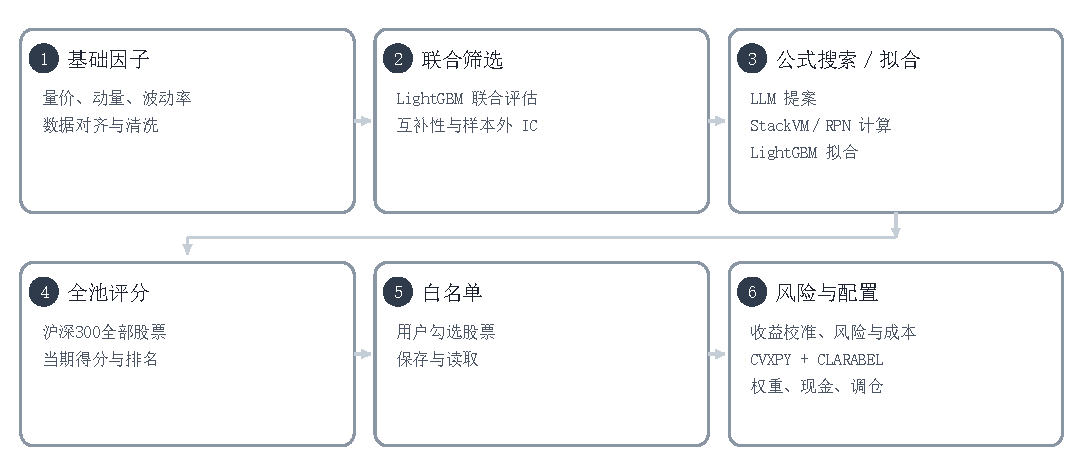
\includegraphics[width=\linewidth]{figs/wingman_pipeline.pdf}\caption{Wingman从因子到配置的处理流程}\label{fig:pipeline}\end{figure}
\subsection{点时数据模型与时间设定}

\subsubsection{研究对象与事件时间}

令$U_t$表示信号日$t$的\textbf{历史有效成分集合}，$G(i,t)$表示当日与股票$i$属于同一行业且输入有效的股票集合。输入除数据值外，还记录事件发生、实际生效、已知、可用、抓取和构建时间。模型使用某条输入的必要条件为


\begin{equation}
 a_{i,t}^{(k)}\leq s_t, \qquad i\in U_t. \tag{1}
\end{equation}

式中，$a_{i,t}^{(k)}$为第$k$类输入的可用时间，$s_t$为信号生成时刻。输入晚到或缺少可用时间，均不能依靠同一自然日的日期标签绕过式(1)。当供应商没有原生可用时间时，项目日线保守政策取当日21:00，并记录其为推导政策而非原生披露时间。（见支撑材料S2）


原始响应先保存为不可变数据，再生成标准化行情、历史成员、行业与执行账本，最后形成冻结快照和文件指纹。训练只读快照；供应商请求与研究运行分离，使重跑不会因接口返回内容变化而悄悄改变样本。


\subsubsection{研究面板与执行账本}

研究面板用于产生\textbf{当日成员的特征和评分}，执行账本则覆盖曾经入选股票的全部可报价日。二者分开，是为了保留成员调出后仍未卖出的旧仓。调出成分后意向目标为0，但若停牌或一字跌停导致无法卖出，仓位、估值和后续盈亏继续留在账上。


复权与总收益序列由冻结原始价格、前收盘链及公司行动账本构建，重点检查历史前缀不随未来数据加入而改变。退市样本也不能直接删除；冻结协议对缺乏可审计处置价格且无法卖出的余额采用明确损失政策，并要求单列敏感性分析。该政策是一项模型设定，应和真实处置证据区分。


\subsubsection{标签与预测周期}

设$O^{TR}_{i,t}$为可审计开盘总收益价格，持有周期$H$以交易日计，则研究标签为


\begin{equation}
 y^{(H)}_{i,t}=\log\frac{O^{TR}_{i,t+H+1}}{O^{TR}_{i,t+1}},\qquad H\in\{1,3,5\}. \tag{2}
\end{equation}

式(2)使信号、入场和收益区间相互对齐。信号使用$t$日输入，入场使用$t+1$日开盘，持有$H$个开盘到开盘区间。标签单独保存，特征模块不得导入；后续指标不能再无依据地多移动一天。收益校准与账户结算明确简单收益和对数收益的转换，没有将两种数值直接混用。


\subsection{因子计算、表达式生成与本地执行}

\subsubsection{因子张量与参照范围}

在输入审核后构建\textbf{股票、特征和时间}三个维度的因子张量。对原始特征$x_{i,t}$，稳健归一化可概括为


\begin{equation}
 z_{i,t}=\operatorname{clip}\!\left(\frac{x_{i,t}-m_{i,t}}{d_{i,t}+10^{-6}},-5,5\right). \tag{3}
\end{equation}

其中$m_{i,t}$为历史窗口中位数，$d_{i,t}$为相对该中位数的绝对偏差中位数，分母常数为数值稳定项。当前代码直接使用MAD，未乘正态一致性系数。式(3)用于解释当前大部分无界基础特征的尺度处理，不能替代每个因子的具体计算定义，也不适用于所有自然有界指标。


上下文因子则强调参照群体。例如，令$r_{i,t}$为个股单日对数收益，\textbf{行业残差}为


\begin{equation}
 e_{i,t}=r_{i,t}-\frac{1}{|G(i,t)\setminus\{i\}|}\sum_{j\in G(i,t)\setminus\{i\}}r_{j,t}. \tag{4}
\end{equation}

式(4)只在同行输入有效且集合非空时定义。它用于减少目标股票对同业均值的自我贡献，不是对所有行业暴露的完整统计消除。


\subsubsection{候选公式的提出与校验}

通用公式引擎采用RD-Agent风格的研究反馈流程，其候选生成器使用大语言模型（LLM）。当前适配器通过硅基流动的聊天接口调用配置指定的DeepSeek模型，模型名称可用环境变量\path{SILICONFLOW_MODEL}设置。输入包含词表、公式约束和可用研究摘要，输出为供本地虚拟机执行的逆波兰表达式词元序列。生成器依据词表、表达式限制、历史研究摘要和允许的反馈提出公式，随后进行结构合法性、栈深、长度、词表版本及执行检查。\textbf{生成器只提出候选}；经济价值由本地数据和固定协议评价。


当前词表由有序注册表派生哈希版本。公式产物加载时必须验证版本，以避免相同编号在不同版本中指向不同特征。虚拟机将合法表达式在本地执行为因子序列，再交给验证单元。


通用生成器的工程默认设置为每轮16个候选、30轮、表达式最多64个词元、结构深度不超过9；单式执行时限8秒、单轮180秒、外部请求90秒并最多重试3次。这些限制约束计算复杂度与故障范围，不等于正式S2搜索预算已经批准。虚拟机要求表达式最终恰好留下一个结果矩阵，并独立保留无效位置掩码；不能因为数值清洗完成就把原本无效的输入变成有效证据。（见支撑材料S5）


S2首版设计从冻结的现有候选开始。动态公式扩展需要单独登记词表、表达式复杂度、生成器与反馈范围，并与特征选择共享搜索预算。离线演示已经提供本地可重放提案和拟合链路；这与调用远程提案服务、运行真实数据研究是不同事实。


\subsection{因子联合筛选与固定模型拟合}

\subsubsection{联合选择的数学对象}

设冻结候选集合为$\mathcal F$，待选子集为$S\subseteq\mathcal F$，固定模型在内层各训练段拟合，在对应验证段产生评分。内层评价可写为


\begin{equation}
 J(S)=\frac{1}{K}\sum_{k=1}^{K}\operatorname{RankIC}_k\bigl(f_{\theta_{k,S}}(X_S),y\bigr). \tag{5}
\end{equation}

这里$K$是内层验证折数，$\theta_{k,S}$只用第$k$折允许的训练数据拟合。RankIC表示评分与后续标签的秩相关，$\operatorname{RankIC}_k$为第$k$折各有效验证日的横截面RankIC均值，并非混合全折所有股票日后计算一次相关。它适合评价相对排序，却不能代替净收益、换手或集中风险检验。


选择过程从冻结初始组出发，逐项评估加入候选后的增量；满足要求后加入，再检查已有成员是否可以回删。对有限的候选对还可整体加入，以允许单项不足而组合有效的情形。所有子集在同一评价支持集、日期、模型和标签口径下比较，避免某个组合通过删去困难样本获得更高分数。


\subsubsection{默认搜索设定与停止条件}

表\ref{tab:t3}给出当前组搜索引擎的工程默认值。正式实验需要将这些值和真实候选清单写入冻结配置；默认值并不自动构成新实验的批准参数。（见支撑材料S3、S5）


\begingroup\fontsize{9.6}{13.3}\selectfont\setlength{\tabcolsep}{2pt}\renewcommand{\arraystretch}{1.15}
\begin{longtable}{@{}>{\raggedright\arraybackslash}p{0.257\linewidth}>{\raggedright\arraybackslash}p{0.190\linewidth}>{\raggedright\arraybackslash}p{0.503\linewidth}@{}}
\caption{因子组搜索引擎默认参数}\label{tab:t3}\\
\toprule
项目 & 默认值 & 含义 \\
\midrule
\endfirsthead

\multicolumn{3}{c}{表\thetable\ （续）}\\\toprule
项目 & 默认值 & 含义 \\
\midrule
\endhead
\bottomrule
\endfoot

候选上限 & 65 & 超过上限的清单需显式调整配置并核算预算。 \\

最终组大小上限 & 5 & 初始组也占用名额。 \\

比较总预算 & 480 & 前向320、回删64、配对96。 \\

配对子集种子上限 & 12 & 有限探索，不等于穷举所有组合。 \\

加入增量阈值 & 0.001 & 要求内层评价增量达到预定阈值。 \\

回删容忍量 & 0.0005 & 控制保留收益很小的冗余成员。 \\

正向折比例 & 0.60 & 要求增量在足够比例的折中同向。 \\

共同覆盖率 & 0.85 & 分母为原始成员日，不能靠删样本提高。 \\

最少内层折数 & 3 & 控制过少时期造成的判断不稳定。 \\

\end{longtable}\endgroup

比较机会包括单项、配对、回删、失败及缓存命中。一次扫描剩余预算不足时停止，不能只评价候选清单前半部分再从中选择“最优”。没有合格组合时保留无候选状态，不强行输出零分或用旧冠军回填。


联合拟合的固定LightGBM基线采用60轮、15叶、学习率0.04、最小叶样本40、单线程等研究配置。这里将模型复杂度固定，是为了把主要比较机会约束在因子组变化上；真实实验会记录实现版本与完整参数，不用外层结果再挑模型参数。\cite{r1}（见支撑材料S5）


\subsubsection{内层、外层与最终模型}

对每个外层折，系统仅在此前训练区间重新执行内层清理、筛选与拟合，固定所得组合后预测接下来的日期。当前S2准入实现限定为5日周期与点时沪深300，原1/3/5日比较用于解释前期设计，不表示S2自动同时启动三个周期。外层不同折选出不同因子是正常现象，应报告选择频率和空组，而不把全开发集挑选出的组合回填到所有历史折。


最终输出必须\textbf{显式选择模型预测或按固定规则等权合成}。前者使用拟合模型的分数，后者使用归一化因子的组合值；二者对应不同策略假设，不能在看到结果后无记录地切换。当前离线拟合演示采用模型预测输出。


历史公式闭环中，验证单元保存覆盖率、方向、相关性、增量和成本诊断，知识记录保存成功与失败假设；只有满足相应准入协议的候选才有资格进入正式保留集合。S2内层选择结果本身不写入正式SOTA。最终开发集重选、候选冻结和一次性Holdout仍是后续独立步骤。


\subsection{全池评分与用户白名单}

设模型在信号日输出$s_{i,t}$。系统首先在完整的当期成员集合中展示证券、得分和有效性，再排序有效评分。缺分股票仍保留展示，不能通过只显示前20名隐藏数据缺口。全池得分属于某个信号日期和模型快照，与股票自身历史IC、组合权重均不同。


用户从展示结果保存集合$W_t$，同时保存所见日期、模型版本和名单版本。研究与评分先于用户选择，因此白名单不会改变上游全池训练样本。跨日期沿用名单时建立新的快照绑定，不把旧分数当作新分数。（见支撑材料S4）


白名单在当前产品中的含义已从简单“允许配置”具体化为“成功推荐时所选股票都要有正目标”。因此，需要用户提供有实际意义的最低权重$m>0$。若选中$n$只股票，则$n m$不能超过预算；同一行业所选股票的最低权重之和也不能超过行业上限。缺分、风险历史不足或约束冲突时，应返回具体原因，而不是悄悄删除所选股票。


\subsection{从分数到收益与风险}

\subsubsection{收益校准}

分数先在当时全池中转换为预先定向的中心化百分位$q_{i,t}\in[-0.5,0.5]$，再使用已经成熟的样本外预测及其收益，建立单调线性映射：


\begin{equation}
 \widehat\mu_{i,t}^{(H)}=\widehat a+\widehat b q_{i,t},\qquad \widehat b\geq0. \tag{6}
\end{equation}

被解释量为与执行口径一致的$H$周期毛总收益减同周期现金收益。校准按日期等权，避免某天证券数量较多而被赋予更大时间权重。默认使用最近504个成熟信号日，至少252日；20日块、2000次抽样估计均值标准误$u_{i,t}$。（见支撑材料S4）


为减少均值估计过于乐观对配置的影响，主方案使用


\begin{equation}
 \widetilde\mu_{i,t}=\widehat\mu_{i,t}^{(H)}-\kappa u_{i,t},\qquad \kappa=1. \tag{7}
\end{equation}

式(7)是决策中的\textbf{保守扣减}，而非具有固定覆盖率的收益下界。校准只使用当时已成熟收益，不能将当前预测窗口的未来收益回流。输入文件声明OOF不等于上游训练天然合规，仍需核验真实折边界和生成过程。


\subsubsection{协方差与风险周期}

\textbf{风险历史}覆盖白名单和所有实际持仓。默认在最近504交易日内构造与$H$一致的非重叠总收益周期，至少保留60个完整共同周期。缺失证券不补零，未来、过期、乱序或维度不匹配的数据被拒绝。


采用Ledoit-Wolf形式的收缩估计：


\begin{equation}
 \widehat\Sigma_H=(1-\delta)S_H+\delta\bar v I,\qquad 0\leq\delta\leq1. \tag{8}
\end{equation}

其中$S_H$为样本协方差，$\bar v$为平均样本方差，$I$为单位矩阵。收缩用于改善有限样本下风险矩阵的条件性质；它不保证预测风险与未来实现风险相同。\cite{r2} 收益、协方差和成本统一在同一个$H$周期及净值比例口径下进入配置。


\subsection{带收益不确定性与交易成本的组合优化}

\subsubsection{优化变量与目标函数}

令$w_i$为推荐目标权重，$w_i^0$为已知当前权重，$c_b,c_s$分别为买入和卖出比例费率，$(x)_+=\max(x,0)$。连续目标模型写为


\begin{equation}
 \max_{\boldsymbol w}\quad \widetilde{\boldsymbol\mu}^{\mathsf T}\boldsymbol w-\lambda\boldsymbol w^{\mathsf T}\widehat\Sigma_H\boldsymbol w-C(\boldsymbol w-\boldsymbol w^0), \tag{9}
\end{equation}

\begin{equation}
 C(\Delta\boldsymbol w)=c_b\sum_i(\Delta w_i)_++c_s\sum_i(-\Delta w_i)_+. \tag{10}
\end{equation}

当前风险厌恶默认$\lambda=3$。当风险矩阵半正定，成本函数为凸函数且约束为凸集时，可将该问题作为凸优化求解，当前实现使用CLARABEL。该思路与收益、风险和交易成本联合决策的经典框架一致。\cite{r3} 优化器分配已有预测信息，不能创造预测能力。


\subsubsection{用户、行业和现金约束}

令$B\leq1$为有效股票预算，$\mathcal I_g$为行业$g$内的证券集合。主目标满足


\begin{equation}
 \begin{aligned}
 &m\leq w_i\leq0.05 &&(i\in W_t),\\
 &w_i=0 &&(i\notin W_t),\\
 &\sum_i w_i\leq B,\qquad \sum_{i\in\mathcal I_g}w_i\leq0.30,\\
 &\boldsymbol w^{\mathsf T}\widehat\Sigma_H\boldsymbol w\leq0.12^2\frac{H}{239}.
 \end{aligned} \tag{11}
\end{equation}

式(11)最后一项将年化12\%的预测波动上限转换到$H$周期，239为当前工程年化交易日口径。该上限约束估计波动，不等于限制未来最大回撤。未取得权威或人工补充行业的证券共用未知行业额度；人工字段不能覆盖已有的版本化权威行业。缺少权威行业时，人工补充内容的依据仍需审计。


意向现金为$1-\sum_iw_i$，其中还需预留本次费用。若给定参数不可行，系统不通过放松单股、行业上限或给所选股票零目标来伪造成功。旧设计中的风险平价、等权、全现金回退链保留为历史方案；当前要求全体所选股票正目标的版本以明确拒绝不可行为准，不能把旧回退当成现行成功路径。（见支撑材料S2、S4）


\subsubsection{费用与配置范围}

默认研究参考费率为买入0.076\%、卖出0.126\%，其中已包含滑点；也可按独立字段输入佣金、税费、过户费、滑点与最低佣金。两种模式不可重复收费。这些是项目模型假设，不代表所有账户或历史时段实际费率相同。


配置区间由$\kappa=0,1,2$三种不确定性扣减分别求解得到，逐股取可行情景中的最小与最大权重。它是情景权重范围，不是收益置信区间；也不能把所有股票的区间上限同时采用，因为各上限可能来自不同完整组合。主推荐仍为$\kappa=1$的可行解。


\subsection{执行细节与状态管理}

\subsubsection{持仓与买卖阻塞}

系统区分持仓未知与已确认空仓。持仓未知时，只能输出条件目标及缺失提示；不能默认从全现金出发计算真实调仓。白名单外旧仓的意向目标为0，但无法卖出的部分仍在执行模拟中占用股票、行业和风险预算。


下一开盘的实际状态用于执行前复核，不回写信号日预测。买入受阻时，保留原正目标并记录零成交；卖出受阻时，保留旧仓及其风险。账户执行状态与推荐目标分别展示，可以出现“目标有效，但完整建仓未完成”。


\subsubsection{小额交易、取整与最低费用}

当前正常调仓的不交易带为0.5个百分点。小额变化先固定为不动，再在剩余可调部分重解；首次配置、强制退出和必要降险不能被该阈值无限期阻止。完整费用重算后，若保守效用未超过保持合法原仓，则允许返回不交易。


有账户金额时，根据证券交易单位向下取整买入数量，再按真实订单重算最低佣金、可卖数量与现金。新开仓还采用20日成交额中位数不低于2000万元、单次交易额不高于20日平均成交额1\%的参考约束。没有账户金额时，只输出比例，不声称完成股数、最低佣金和容量复核。


连续模型的可行解不一定对应离散订单可行解。取整后某只所选股票预计持仓为0，须报告用户完整建仓要求尚未满足。最低佣金与交易单位引入离散性，当前流程采用连续求解加确定性复核，不宣称离散全局最优。


\subsubsection{不可变记录与接口输出}

评分、名单、分析证据和方案以版本绑定保存；方案生成后保持不可变，采纳、未采纳、执行观察、净值与备注作为后续事件追加。观察日期需有时区并满足时序约束。净值变化可能包含出入金，因此不能未经处理直接归因于算法。


离线接口使用明确的状态和失败原因，数据不足、所选缺分、最低仓位预算冲突等均返回结构化说明。当前正式建议仍受模型未验证状态约束。保存了文件、页面可用、算法返回了权重，分别只说明对应工程步骤完成。


\section{验证设计、已有结果与误差分析}

\subsection{时间隔离与验证口径}

当前正式沪深300冻结设计按完整交易日期划分数据，同一天全部股票进入同一角色。协议采用5个扩展窗口的外层验证折、20交易日剔除间隔和5日隔离期；训练标签的结束时间还必须早于后续验证信号时间。封存测试段从尾部取至少10\%且不少于480个交易日，并至少覆盖两个日历年。（见支撑材料S2）


S2仍需冻结真实的内外层日期清单，不能仅写“5折”代替可执行分割。通用旧训练入口的默认切分与该正式沪深300协议不同，复现时必须按具体路线读取配置，而不能将不同路径的参数拼接成一场不存在的实验。


预测验证之后，交易评价使用统一执行账本与成本假设。冻结研究比较采用20日移动块、2000次配对Bootstrap和95\%区间；旧周期比较使用Holm家族校正，公式研究另有多重比较约束。S2还须补齐针对完整搜索流程的比较家族与集中风险判定，不能把局部因子检验当作全流程显著性控制。反复查看开发集后改变方案的尝试，需要累计登记。\cite{r4}（见支撑材料S3）


\subsection{数据、模型与执行的分层校验}

数据层首先检查可用时点、历史成员区间、行业变更、总收益链和未来哨兵；加入未来行之后，过去特征不应变化。研究层检查外层标签改动是否影响本折选择、所有候选是否使用相同支持集、无候选是否被正确保留，以及缓存和重启是否重置预算。


配置层检查所选股票全部正目标、未选股票意向目标为0、行业和波动限额、费用预留、旧仓阻塞及股数取整。执行层核对实际模拟持仓、现金和费用守恒：


\begin{equation}
 \text{预计股票市值}+\text{预计现金}+\text{本次费用}=\text{调仓前净值}. \tag{12}
\end{equation}

式(12)在一致的执行计价基准下使用，收益再于后续持有区间结算。价格变化、账户出入金和成交状态若另有时点，必须单独记账，不能混入同一个静态等式。


\subsection{已有证据及其支持范围}

本文没有为写作重新搜索策略或读取封存测试集，而是核对已保存实现和实验记录。表\ref{tab:t4}列出能够直接支撑本文结论的证据；工程成功与经济有效性分别表述。


\begingroup\fontsize{9.6}{13.3}\selectfont\setlength{\tabcolsep}{2pt}\renewcommand{\arraystretch}{1.15}
\begin{longtable}{@{}>{\raggedright\arraybackslash}p{0.190\linewidth}>{\raggedright\arraybackslash}p{0.351\linewidth}>{\raggedright\arraybackslash}p{0.408\linewidth}@{}}
\caption{已有工程证据与结论边界}\label{tab:t4}\\
\toprule
证据对象 & 已保存结果 & 能够支持的结论 \\
\midrule
\endfirsthead

\multicolumn{3}{c}{表\thetable\ （续）}\\\toprule
证据对象 & 已保存结果 & 能够支持的结论 \\
\midrule
\endhead
\bottomrule
\endfoot

基础词表 & 65项基础因子；当前词表哈希版本为v9217a2c0d91a & 候选接口和有序注册范围可核验，不能证明所有因子有效。 \\

9月15日离线联合拟合示例 & 合成数据上真实LightGBM拟合，输出640条评分 & 筛选、拟合及评分产物接口已贯通；不代表真实65+8候选研究通过。 \\

9月17日配置示例 & 300只合成证券、冻结线性公式、504个成熟校准日、100个非重叠风险周期 & 可演示完整评分、白名单、收益风险估计和组合配置；不是前一LightGBM模型的市场应用。 \\

配置工程验收记录 & 最新实施文档记录101项相关测试通过 & 所覆盖接口与约束已接受工程验证；本文未将其他批次测试累加为新增证据。 \\

配置回放记录 & 优化、受约束等权、受约束逆波动，分别取成本0、1、1.5倍，共9组；每组5日 & 回放链条可运行，但仅一个折、一个相位，结论为证据不足。 \\

正式研究状态 & 真实市场五折全相位配置验证尚未完成；正式建议为模型未验证 & 当前不具备“已经证实优于等权”或“允许正式交易建议”的结论。 \\

\end{longtable}\endgroup

表\ref{tab:t4}中的两个合成示例用于不同模块，不能拼接成同一策略的连续投资实证。尤其是5日工程回放，即使程序计算了年化指标，样本量也不足以解释长期收益或统计优势，本文不据此报告策略优胜幅度。（见支撑材料S4、S7）


\subsection{误差来源与必要的稳健性研究}

误差首先来自数据：可用时间推导、行业覆盖不足、停牌及公司行动处理不一致，会改变可用样本和收益口径。其次来自模型：候选搜索次数、共线特征、低覆盖共同支持、均值校准不稳定和协方差估计误差，都可能使开发集表现高估。再次来自执行：连续权重与股数订单、固定参考成本与实际冲击、目标退出与受阻旧仓之间均存在差距。


当前配置已经提供1.5倍费用、最大行业同步下跌10\%、买入全部受阻、卖出全部受阻等方案压力场景。这些场景检查具体方案受冲击后的状态，不等同于长期历史稳健性。真实研究还应在统一名单和执行口径下比较优化器、等权、逆波动及适用的保持原仓对照，完成全部相位、多个外层折、年份和行业依赖检验。


稳健性研究的阈值与失败动作应在运行前确定。缺少完整风险暴露匹配、最强年份或最大行业剔除的独立重跑时，应保留证据不足，而非用“结果已披露”替代是否通过的判定。


\section{模型评价与推广}

\subsection{设计的主要优点}

第一，研究对象、用户选择和账户决策具有明确边界。共享公式在全池学习和评分，用户控制可配置范围，配置模型负责资金分配，使不同用户能够共享研究成果而保留各自的选择。


第二，时间语义被写入输入和标签合同。可用时间、历史成分、执行账本、成员退出和封存测试集隔离，使研究结论能够追溯到当时的信息条件，减少依靠事后过滤改善结果的空间。


第三，联合研究允许因子互补，又通过有限搜索、预算登记和外层评价限制选择自由度。其价值在于建立可检验流程，而不是预先保证一定找到优胜策略。


第四，组合目标将收益估计误差、共同风险和交易费用放在统一周期中处理。正目标约束、不可行报告、目标与成交分开记录，使用户偏好和实际账户约束可以被直接核验。


\subsection{当前局限与适用边界}

现阶段最主要的局限是\textbf{有效性证据不足}。已有300证券界面和优化示例基于合成输入，正式S2真实候选、风险判定及交易评价尚未完整冻结并运行。代码保存状态字段只是行为声明，不能代替调用链和数据访问审计。


其次，基础因子存在近似定义和实现差异。例如，部分波动与价格冲击指标采用简化口径，单品种模式中的截面因子可能重复，WILLR\_14存在退化问题。正式研究前需要在冻结候选清单中逐项审计，不能仅凭注册数量判断因子质量。


再次，当前配置是单周期连续优化加执行复核。它没有完整模拟日常股数撮合、所有真实停复牌与涨跌停事件，也没有自动行情驱动的连续影子账户。行业30\%限额和协方差惩罚属于分散及风险控制，不能称为已经消除行业β或完成多空对冲。


\subsection{尚待论证的问题}

以下问题是当前模型仍缺少充分证据的研究事项。本文提出可检验的分析方向，相关实验尚未在本次写作中执行；判断阈值也不因写入论文而视为已经冻结。


\subsubsection{头部依赖：收益是否依靠少数股票、行业或时期}

Knez和Ready说明，极端观测会影响规模溢价的估计；Bessembinder则从长期财富创造角度揭示了个股收益贡献的高度集中。\cite{r6,r7} Wingman观测到去除龙头后公式对其他股票的关联性降低。


整体收益为正，可能主要来自少数赢家。需要区分三类头部：评分乘以后续标签形成的信号贡献代理、真实持仓扣费后的收益贡献，以及单行业或特定时期的集中贡献。代理值便于诊断预测结构，但不等于账户实际赚到的钱。


下一步应同时报告收益贡献集中度、持仓集中度、最大行业暴露和跨年份稳定性，并实施头部剔除后的独立交易回放。剔除组须与规模、行业、流动性及剔除比例相近的随机或匹配对照比较；同时检查剩余组合的暴露和现金变化。事后删除赢家本来就会降低收益，单凭“删后变差”不足以判定失败，必须事先明确可接受依赖程度及对应动作。


应分别保留“在该样本中发现集中现象”和“已证明未来收益脆弱”两个层次。现有头部诊断只能提出需要进一步解释的依赖问题，尚不能为新S2给出完整、已验证的接受标准。


\subsubsection{沪深300因子库的时效性与向中证500的迁移能力}

Wingman想要观察因子库和公式的时效性，但数据集容量不足，作者认为不够求得时效性后又拿去拟合验证。于是提出猜想：能否在沪深300的数据集里得到该因子库的时效性，这个时效性可不可以推广到其他组合中例如中证500。


Fama和French按规模组检验异常，Hou等重新检验大量异常，均表明样本构成和组合构造会影响结果。\cite{r8,r9} Liu等对中国市场规模与价值因子的研究进一步提示，市场制度及股票范围会改变因子解释。\cite{r10} 这些文献支持开展跨池检验，但没有证明沪深300与中证500具有相同的因子时效性。


同一因子库在沪深300拟合得到的当前候选，不能自然称为对所有股票池都成立的“最优策略”。训练目标、股票规模、行业构成、流动性、换手与交易冲击变化后，同一计算表达式的分布和预测关系都可能改变。因子名称和实现相同，并不意味着有效方向、强度或有效期相同。


建议先在沪深300内部研究时间上的稳定性：按历史顺序重复训练与后续评价，观察因子的方向、增量、校准误差及扣费贡献如何变化。然后冻结规则，进入中证500检验迁移。应区分“模型和参数完全冻结后直接应用”与“按预先规定的方法、仅用中证500此前数据重新拟合”两种实验；前者检验固定模型迁移，后者检验研究流程迁移，不能混称同一种泛化能力。


迁移实验需使用中证500历史点时成员和适用的成本、交易约束，并保持比较日期、信息可用时点及评价口径可比。同一股票可能随时间跨池变动，应单列证券重叠情况和不重叠样本，防止把时间迁移、同一证券复用与真正跨股票池迁移混在一起。在此之前，不能推断两池因子的时效性一致。


\subsubsection{训练股票如何选取，以及行业β如何识别}

Moskowitz和Grinblatt研究行业动量，Asness等将公司特征区分为行业内和行业间分量，为识别行业共同影响提供了参照。\cite{r11,r12} Daniel等讨论特征组合中的风险暴露及对冲，说明按特征选股与控制共同风险是不同任务。\cite{r13} 因此，训练样本的行业结构和行业风险控制方法应分别设计并检验。


\textbf{“同一行业选50只”和“跨行业选50只头部股票”对应不同研究目标}。同业样本有助于比较相对行业的个股差异，但其共同涨跌仍可能具有强烈行业暴露；样本数量变多不会自动消除行业β。跨行业样本能增加行业变化，却可能同时引入市值、龙头地位、流动性和风格偏差，也不天然等于识别行业β。


例如，可以将收益解释框架写成$r_{i,t}=\alpha_i+\beta_{i,m}r_{m,t}+\beta_{i,g}r_{g,t}+\epsilon_{i,t}$，其中市场与行业β表示对相应共同收益的暴露。该式是待检验的分析框架，并非当前配置代码已完成的估计模块。行业内减均值能减少共同分量，却不保证残余β为零；在单一行业样本中，市场与行业收益高度相关时，也可能难以稳定分辨两种暴露。


建议采用等样本量、同历史区间和相同搜索预算的对照：行业内抽样、按行业分层抽样、跨行业规模或流动性匹配抽样，并以更完整的点时股票池作为参考。所谓“头部”须用当时已知的市值或成交额定义，不能按未来收益挑选。若某行业不足50只有效证券，应如实记录，不用未来成分补足。最终根据行业暴露、行业内预测增量、样本外净收益和稳定性评价素材选择，而不是先假定某种50只股票组合能够解决行业β。


\subsubsection{因子选择、更新与停用规则的跨阶段研究}

规则更新不仅改变预测模型，也会改变交易频率。Novy-Marx和Velikov研究异常策略的交易成本及缓解方法，说明更新规则应按扣费后的效果评价。\cite{r14} 同时，每次尝试不同窗口或停用阈值都属于新的选择机会，应结合回测过拟合问题记录完整研究路径。\cite{r4}


\textbf{更值得迁移的对象可能是一套规则，而非一次性得到的固定因子组}。可以将每个更新时点的决策表示为$S_t=\mathcal A(D_{\leq t},S_{t-1})$：规则$\mathcal A$仅使用当时已可得且标签已经成熟的数据，决定保留、加入、降权或停用哪些因子。规则需预先规定训练窗口、更新频率、搜索预算、覆盖要求、交易成本和状态切换条件。


评价时应把这套更新机制整体放进外层时间回放，统计净收益、变更次数、换手成本、无因子时段、停用延迟与错误停用，而不能事后为每段历史分别挑选最好的因子，再把这些片段拼接成一条曲线。固定因子组与按固定频率重拟合可作为对照，以检验更复杂的更新规则是否提供增量。


在沪深300形成冻结规则后，可进一步在其他历史点时股票池检验迁移。若进入新股票池后调整了阈值、窗口或更新频率，应登记为新的适配实验；其结果不能再作为原冻结规则未经修改的迁移证据。


\subsubsection{策略有效期如何判定}

McLean和Pontiff比较预测信号在原样本外及论文发表后的表现，发现收益可预测性会衰减。\cite{r15} 该研究提示应把数据挖掘与市场参与者学习纳入解释，但并未给出适用于所有策略的统一寿命；Wingman仍需建立自己的持续监控和停用证据。


策略有效期不宜预先写成统一的若干天或若干月。\textbf{需要区分预测持有周期、模型更新间隔和经济有效性持续时间}：5日标签只定义单次收益观察区间，并不意味着策略5日后必然失效；短期回撤也不足以直接证明长期结构已经失效。


可将有效性监控分为数据可用性、预测区分度、收益校准、成本后增量和风险依赖几个维度。利用成熟标签和实际可观察结果形成滚动证据，在事前固定的规则下触发继续观察、降低使用强度、重新研究或停用。监控指标、窗口和连续触发条件都需用独立历史区间评价误报率、漏报和检测延迟；反复监控带来的多次判断机会也应计入。


最终能够报告的是“该冻结规则在某些历史区间仍满足何种标准、从何时起证据不足或触发停用”，而非保证未来还能有效多久。样本结束时仍未触发停用的策略只有截至观察终点的持续记录，不能据此给出完整寿命。系统目前尚缺少这套经过历史与跨池检验的持续有效性判据。


\subsection{推广方向}

推广宜围绕可迁移的研究规则与数据合同进行。首先补齐真实候选清单、集中风险接受规则和完整执行评价；其次在沪深300内检验因子时效与更新机制；最后按冻结规则评估中证500等其他股票池的迁移能力。跨池时保持时间因果原则与证据版本管理，重新核验成员、行业、流动性和交易单位等输入条件。


若未来扩展到其他市场或资产，标签价格、交易日历、成本、卖空权限和风险预算都需单独定义。模型模块可复用并不意味着原市场结论能够直接沿用。


\section{结论}

本文围绕Wingman的用途、设计流程、运作细节与参数设定，建立了从可审计数据到用户白名单配置的系统说明。系统通过因子与公式执行、联合筛选和拟合、分数校准、协方差风险估计与受约束优化，把预测能力、用户选择和账户执行连接为可追溯链条。


当前可证实的成果是基础与上下文候选接口、离线联合拟合及300只合成证券配置流程的工程实现；现有短回放不足以支持真实市场经济有效性结论。头部依赖、训练股票池、因子时效性、跨池迁移、动态更新停用与策略有效期，均应作为后续独立研究问题。只有在完整时间隔离、交易成本和风险判定下验证这些机制，才能进一步讨论正式发布及持续使用。


\begin{thebibliography}{99}\small\raggedright\setlength{\itemsep}{.4em}
\bibitem{r1} KE G, MENG Q, FINLEY T, et al. LightGBM: A Highly Efficient Gradient Boosting Decision Tree[C]. Advances in Neural Information Processing Systems 30, 2017. \href{https://www.microsoft.com/en-us/research/project/lightgbm/publications/}{微软研究院论文记录}.

\bibitem{r2} LEDOIT O, WOLF M. A well-conditioned estimator for large-dimensional covariance matrices[J]. Journal of Multivariate Analysis, 2004, 88(2): 365-411. DOI: 10.1016/S0047-259X(03)00096-4. \href{https://doi.org/10.1016/S0047-259X(03)00096-4}{原始出版记录}.

\bibitem{r3} BOYD S, BUSSETI E, DIAMOND S, et al. Multi-Period Trading via Convex Optimization[J]. Foundations and Trends in Optimization, 2017, 3(1): 1-76. \href{https://web.stanford.edu/~boyd/papers/cvx_portfolio.html}{作者论文页面}.

\bibitem{r4} BAILEY D H, BORWEIN J M, LÓPEZ DE PRADO M, ZHU Q J. The Probability of Backtest Overfitting[R]. \href{https://www.davidhbailey.com/dhbpapers/backtest-prob.pdf}{作者公开论文}，2015年预印本.

\bibitem{r5} LI Y, YANG X, YANG X, et al. R\&D-Agent-Quant: A Multi-Agent Framework for Data-Centric Factors and Model Joint Optimization[R]. 2025, arXiv:2505.15155. \href{https://arxiv.org/abs/2505.15155}{论文原文}.

\bibitem{r6} KNEZ P J, READY M J. On the Robustness of Size and Book-to-Market in Cross-Sectional Regressions[J]. The Journal of Finance, 1997, 52(4): 1355-1382. \href{https://doi.org/10.1111/j.1540-6261.1997.tb01113.x}{原始出版记录}.

\bibitem{r7} BESSEMBINDER H. Do Stocks Outperform Treasury Bills?[J]. Journal of Financial Economics, 2018, 129(3): 440-457. \href{https://doi.org/10.1016/j.jfineco.2018.06.004}{原始出版记录}.

\bibitem{r8} FAMA E F, FRENCH K R. Dissecting Anomalies[J]. The Journal of Finance, 2008, 63(4): 1653-1678. \href{https://doi.org/10.1111/j.1540-6261.2008.01371.x}{原始出版记录}.

\bibitem{r9} HOU K, XUE C, ZHANG L. Replicating Anomalies[J]. The Review of Financial Studies, 2020, 33(5): 2019-2133. \href{https://doi.org/10.1093/rfs/hhy131}{原始出版记录}.

\bibitem{r10} LIU J, STAMBAUGH R F, YUAN Y. Size and Value in China[J]. Journal of Financial Economics, 2019, 134(1): 48-69. \href{https://www.mingshiim.com/static/sizevaluechina.pdf}{论文原文}.

\bibitem{r11} MOSKOWITZ T J, GRINBLATT M. Do Industries Explain Momentum?[J]. The Journal of Finance, 1999, 54(4): 1249-1290. \href{https://doi.org/10.1111/0022-1082.00146}{原始出版记录}.

\bibitem{r12} ASNESS C S, PORTER R B, STEVENS R L. Predicting Stock Returns Using Industry-Relative Firm Characteristics[R]. 2000, SSRN 213872. \href{https://www.aqr.com/Insights/Research/Working-Paper/Predicting-Stock-Returns-Using-IndustryRelative-Firm-Characteristics}{作者机构论文}.

\bibitem{r13} DANIEL K, MOTA L, ROTTKE S, SANTOS T. The Cross-Section of Risk and Returns[J]. The Review of Financial Studies, 2020, 33(5): 1927-1979. \href{https://www.kentdaniel.net/research.php}{作者论文记录}.

\bibitem{r14} NOVY-MARX R, VELIKOV M. A Taxonomy of Anomalies and Their Trading Costs[J]. The Review of Financial Studies, 2016, 29(1): 104-147. \href{https://doi.org/10.1093/rfs/hhv063}{原始出版记录}.

\bibitem{r15} MCLEAN R D, PONTIFF J. Does Academic Research Destroy Stock Return Predictability?[J]. The Journal of Finance, 2016, 71(1): 5-32. \href{https://doi.org/10.1111/jofi.12365}{原始出版记录}.

\end{thebibliography}
\section*{支撑材料}\raggedright
[S1] Wingman项目. 研究原则与目标架构[EB/OL]. \textnormal{docs/01\_研究原则.md}，工作区版本核对日期：2026-09-17.


[S2] Wingman项目. 阶段2冻结设计[EB/OL]. \path{docs/implementation_gates_20260825/frozen_design.md}，2026-08-25起冻结，含后续版本说明.


[S3] Wingman项目. 阶段4/5联合研究计划S2[EB/OL]. \path{docs/implementation_gates_20260825/joint_research_s2_20260915.md}，2026-09-15.


[S4] Wingman项目. 白名单配置优化：实现与验收[EB/OL]. \path{docs/implementation_gates_20260825/portfolio_optimizer_implementation_20260917.md}；配置规则审核记录\path{portfolio_rules_review_20260917.md}，2026-09-17.


[S5] Wingman项目. 因子、词表、联合搜索及配置源代码[CP]. \path{model_core/features.py}，\path{model_core/vocab.py}，\path{model_core/rd_agent_generator.py}，\path{factor_research/group_search.py}，\path{factor_research/config.py}，\path{strategy_manager/portfolio_models.py}及\path{portfolio_optimization.py}，核对日期：2026-09-17.


[S6] Wingman项目. 沪深300上下文候选特征表达式[EB/OL]. \textnormal{docs/04\_沪深300候选特征表达式.md}；实现：\path{research_stage3/candidate_features.py}，版本hs300\_context\_candidates\_v1.


[S7] Wingman项目. 离线示例产物与配置回放报告[DS]. \path{experiments/offline_demo_factors_20260915_r1/manifest.json}；\path{experiments/offline_demo_optimizer_300_20260917/manifest.json}；\path{experiments/offline_demo_optimizer_validation_20260917_r1/validation_report.json}.


[S8] Wingman项目. 头部依赖诊断草案与前期文献线索. \path{docs/implementation_gates_20260825/head_dependence_diagnostic_draft.md}。用于回查研究问题和既有文献；论文著录以原始出版记录为准。


\end{document}